\pc{2}{24/1}

\question Design B\"uchi automata that recognises the
following languages over $\{0,1,2\}$:
\begin{parts}
    \part the language of strings containing infinitely
    many $1$s and $2$s but finitely many $0$s; 
    \begin{solution}
        \begin{center}
            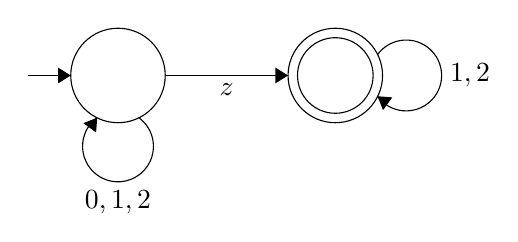
\begin{tikzpicture}[scale=0.2]
                \tikzstyle{every node}+=[inner sep=0pt]
                \draw [black] (10.2,-26.4) circle (3);
                \draw [black] (24,-26.4) circle (3);
                \draw [black] (24,-26.4) circle (2.4);
                \draw [black] (4.5,-26.4) -- (7.2,-26.4);
                \fill [black] (7.2,-26.4) -- (6.4,-25.9) -- (6.4,-26.9);
                \draw [black] (11.523,-29.08) arc (54:-234:2.25);
                \draw (10.2,-33.65) node [below] {$0,1,2$};
                \fill [black] (8.88,-29.08) -- (8,-29.43) -- (8.81,-30.02);
                \draw [black] (13.2,-26.4) -- (21,-26.4);
                \fill [black] (21,-26.4) -- (20.2,-25.9) -- (20.2,-26.9);
                \draw (17.1,-26.9) node [below] {$z$};
                \draw [black] (26.68,-25.077) arc (144:-144:2.25);
                \draw (31.25,-26.4) node [right] {$1,2$};
                \fill [black] (26.68,-27.72) -- (27.03,-28.6) -- (27.62,-27.79);
            \end{tikzpicture}
        \end{center}        
    \end{solution}

    \part the language of strings such that after 
    every occurence of $1$ there is an occurence of $2$; and
    \begin{solution}
        \begin{center}
            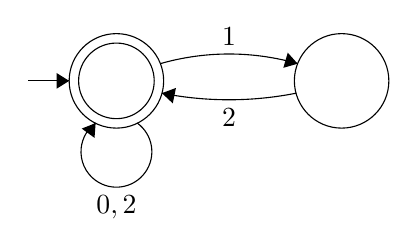
\begin{tikzpicture}[scale=0.2]
                \tikzstyle{every node}+=[inner sep=0pt]
                \draw [black] (8.7,-27) circle (3);
                \draw [black] (8.7,-27) circle (2.4);
                \draw [black] (23,-27) circle (3);
                \draw [black] (3.1,-27) -- (5.7,-27);
                \fill [black] (5.7,-27) -- (4.9,-26.5) -- (4.9,-27.5);
                \draw [black] (10.023,-29.68) arc (54:-234:2.25);
                \draw (8.7,-34.25) node [below] {$0,2$};
                \fill [black] (7.38,-29.68) -- (6.5,-30.03) -- (7.31,-30.62);
                \draw [black] (11.489,-25.906) arc (105.98952:74.01048:15.833);
                \fill [black] (20.21,-25.91) -- (19.58,-25.21) -- (19.3,-26.17);
                \draw (15.85,-24.79) node [above] {$1$};
                \draw [black] (20.106,-27.783) arc (-78.78896:-101.21104:21.892);
                \fill [black] (11.59,-27.78) -- (12.28,-28.43) -- (12.48,-27.45);
                \draw (15.85,-28.7) node [below] {$2$};
            \end{tikzpicture}
        \end{center}
    \end{solution}

    \part the language of strings such that there
    are an even number of $0$s between any two occurences
    of $1$.
    \begin{solution}
        If $0$ is even then
        \begin{center}
            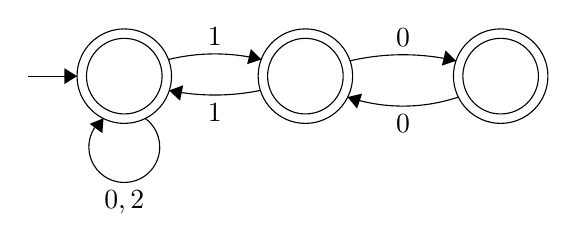
\begin{tikzpicture}[scale=0.2]
                \tikzstyle{every node}+=[inner sep=0pt]
                \draw [black] (11.1,-24.6) circle (3);
                \draw [black] (11.1,-24.6) circle (2.4);
                \draw [black] (22.6,-24.6) circle (3);
                \draw [black] (22.6,-24.6) circle (2.4);
                \draw [black] (35,-24.6) circle (3);
                \draw [black] (35,-24.6) circle (2.4);
                \draw [black] (5,-24.6) -- (8.1,-24.6);
                \fill [black] (8.1,-24.6) -- (7.3,-24.1) -- (7.3,-25.1);
                \draw [black] (12.423,-27.28) arc (54:-234:2.25);
                \draw (11.1,-31.85) node [below] {$0,2$};
                \fill [black] (9.78,-27.28) -- (8.9,-27.63) -- (9.71,-28.22);
                \draw [black] (13.9,-23.543) arc (103.74903:76.25097:12.412);
                \fill [black] (19.8,-23.54) -- (19.14,-22.87) -- (18.9,-23.84);
                \draw (16.85,-22.69) node [above] {$1$};
                \draw [black] (19.746,-25.505) arc (-78.37928:-101.62072:14.375);
                \fill [black] (13.95,-25.51) -- (14.64,-26.16) -- (14.84,-25.18);
                \draw (16.85,-26.3) node [below] {$1$};
                \draw [black] (25.433,-23.628) arc (103.13021:76.86979:14.822);
                \fill [black] (32.17,-23.63) -- (31.5,-22.96) -- (31.27,-23.93);
                \draw (28.8,-22.74) node [above] {$0$};
                \draw [black] (32.32,-25.927) arc (-71.43937:-108.56063:11.057);
                \fill [black] (25.28,-25.93) -- (25.88,-26.66) -- (26.2,-25.71);
                \draw (28.8,-27) node [below] {$0$};
            \end{tikzpicture}
        \end{center}
        otherwise
        \begin{center}
            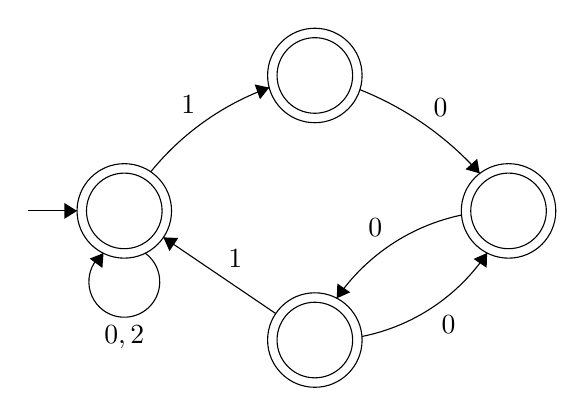
\begin{tikzpicture}[scale=0.2]
                \tikzstyle{every node}+=[inner sep=0pt]
                \draw [black] (11.1,-24.6) circle (3);
                \draw [black] (11.1,-24.6) circle (2.4);
                \draw [black] (23.2,-16) circle (3);
                \draw [black] (23.2,-16) circle (2.4);
                \draw [black] (35.5,-24.6) circle (3);
                \draw [black] (35.5,-24.6) circle (2.4);
                \draw [black] (23.2,-32.8) circle (3);
                \draw [black] (23.2,-32.8) circle (2.4);
                \draw [black] (5,-24.6) -- (8.1,-24.6);
                \fill [black] (8.1,-24.6) -- (7.3,-24.1) -- (7.3,-25.1);
                \draw [black] (12.423,-27.28) arc (54:-234:2.25);
                \draw (11.1,-31.85) node [below] {$0,2$};
                \fill [black] (9.78,-27.28) -- (8.9,-27.63) -- (9.71,-28.22);
                \draw [black] (12.779,-22.118) arc (140.93545:109.8707:17.239);
                \fill [black] (20.3,-16.77) -- (19.38,-16.57) -- (19.72,-17.51);
                \draw (15.17,-18.43) node [above] {$1$};
                \draw [black] (26.059,-16.899) arc (68.29605:41.78246:20.259);
                \fill [black] (33.67,-22.22) -- (33.51,-21.29) -- (32.77,-21.96);
                \draw (31.18,-18.62) node [above] {$0$};
                \draw [black] (24.589,-30.149) arc (145.60728:101.77286:12.765);
                \fill [black] (24.59,-30.15) -- (25.45,-29.77) -- (24.63,-29.21);
                \draw (27.04,-26.24) node [above] {$0$};
                \draw [black] (20.72,-31.12) -- (13.58,-26.28);
                \fill [black] (13.58,-26.28) -- (13.97,-27.15) -- (14.53,-26.32);
                \draw (18.15,-28.2) node [above] {$1$};
                \draw [black] (34.144,-27.268) arc (-33.81931:-78.80056:12.504);
                \fill [black] (34.14,-27.27) -- (33.28,-27.65) -- (34.11,-28.21);
                \draw (31.69,-31.21) node [below] {$0$};
            \end{tikzpicture}
        \end{center}
    \end{solution}
\end{parts}

\question Show that the language over $\{0,1\}$ consisting
of words with finitely many $1$s cannot be recognised by
any deterministic B\"uchi automaton.
\begin{solution}
    A language can be recognised by a deterministic B\"uchi automaton
    if and only if it is a limit of a regular language.
    If there is a finite amount of $1$s and $0$s in ours language, then
    the remaining is an infinite amount of $0$s
    then there is not an infinite amount of prefixes to make
    up our language.
\end{solution}

\question Design a B\"uchi automaton over $\{0,1,2\}$
that accepts precisely the words that contain infinitely
many $01$ and $02$ but finitely many $12$.
\begin{solution}
    \begin{center}
        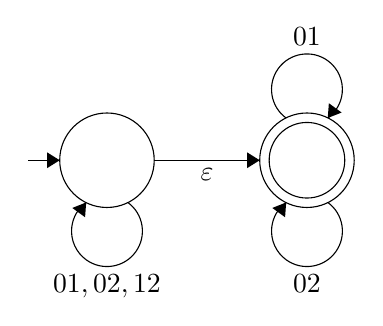
\begin{tikzpicture}[scale=0.2]
            \tikzstyle{every node}+=[inner sep=0pt]
            \draw [black] (8.9,-26.5) circle (3);
            \draw [black] (21.6,-26.5) circle (3);
            \draw [black] (21.6,-26.5) circle (2.4);
            \draw [black] (3.9,-26.5) -- (5.9,-26.5);
            \fill [black] (5.9,-26.5) -- (5.1,-26) -- (5.1,-27);
            \draw [black] (20.277,-23.82) arc (234:-54:2.25);
            \draw (21.6,-19.25) node [above] {$01$};
            \fill [black] (22.92,-23.82) -- (23.8,-23.47) -- (22.99,-22.88);
            \draw [black] (22.923,-29.18) arc (54:-234:2.25);
            \draw (21.6,-33.75) node [below] {$02$};
            \fill [black] (20.28,-29.18) -- (19.4,-29.53) -- (20.21,-30.12);
            \draw [black] (11.9,-26.5) -- (18.6,-26.5);
            \fill [black] (18.6,-26.5) -- (17.8,-26) -- (17.8,-27);
            \draw (15.25,-27) node [below] {$\varepsilon$};
            \draw [black] (10.223,-29.18) arc (54:-234:2.25);
            \draw (8.9,-33.75) node [below] {$01,02,12$};
            \fill [black] (7.58,-29.18) -- (6.7,-29.53) -- (7.51,-30.12);
        \end{tikzpicture}
    \end{center}
\end{solution}
